\documentclass[svgnames, handout, aspectratio = 1610]{beamer}
\linespread{1.2}
\usepackage[compatibility = false]{caption}
\usepackage{graphicx, mathtools, tikz, menukeys, fixdif, physics3,
            lmodern, CJKutf8, url, microtype, bm}
\usephxmodu{operator}
\usepackage[version = 4]{mhchem}
\usepackage[mono = false]{libertine}
\graphicspath{{./media/}}
\usetheme[logobg = westlake-logo.pdf,
          lbadge = westlake-badge.pdf,
          mainbg = westlake-paint-a.png,
          basebg = westlake-paint-b.png]{westlake}
\usepackage{zref-clever, zref-titleref}
\usepackage[natbib, style = phys, biblabel = brackets, sorting = none]{biblatex}
\addbibresource{reference.bib}
\setlength \abovedisplayskip {6pt}
\setlength \belowdisplayskip {6pt}

\title[Final Project Presentation]{Band Structure of 2D Kagome Lattice via Finite Element Analysis}
\author[Mingyu Xia]{\texorpdfstring{Mingyu Xia (夏明宇) |
                    \textit{Department of Physics, Westlake University}}
                      {Mingyu Xia}}
\date{\texttt{2026-04-21 | E10-306@Yungu Campus}}

\begin{document}

\begin{CJK*}{UTF8}{gbsn}
\maketitle
\end{CJK*}

\section{INTRODUCTION TO FEA}

\begin{frame}{Core Philosophy: The "Divide and Conquer" Approach}
  \begin{block}{From Continuous to Discrete}
    FEA is a numerical strategy to solve complex PDEs by approximating a continuous domain $\Omega$ with a collection of simple sub-domains called \textbf{elements} ($\Omega_e$).
  \end{block}
  \begin{columns}
    \begin{column}{.6\linewidth}
      \begin{itemize}
        \item \textbf{Complex Geometry:} Handled by fitting the mesh to the boundary.
        \item \textbf{Local Basis:} Instead of global functions, we use local "piecewise" polynomials.
        \item \textbf{Nodal Representation:} The field (e.g., $\psi$) is solved only at specific points (nodes).
      \end{itemize}
    \end{column}
    \hfill
    \begin{column}{.36\linewidth}
      \centering
      
      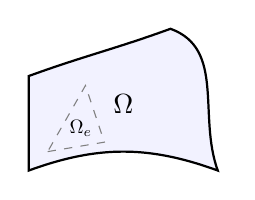
\begin{tikzpicture}[scale=1.2]
        \draw[thick, fill=blue!5] (0,0) to[out=20, in=160] (2,0) to[out=110, in=-20] (1.5,1.5) to[out=200, in=20] (0,1) -- cycle;
        \node at (1,0.7) {$\Omega$};
        \draw[dashed, gray] (0.2,0.2) -- (0.8,0.3) -- (0.6,0.9) -- cycle;
        \node[scale=0.7] at (0.55,0.45) {$\Omega_e$};
      \end{tikzpicture}
    \end{column}
  \end{columns}
\end{frame}

\begin{frame}{Mathematical Principle: The Weak Formulation}
  \begin{block}{From Differential to Integral}
    Instead of solving the Schrödinger equation $\mathcal{H}\psi = E\psi$ directly at every point, FEA satisfies it \textbf{on average} using the Method of Weighted Residuals.
  \end{block}
  \pause
  \begin{itemize}
    \item \textbf{Residual Definition:} $R = (\mathcal{H} - E)\psi$. We want $R \to 0$.
    \item \textbf{Weighting (Galerkin):} We multiply $R$ by a test function $v$ and integrate over the domain:
    \begin{equation}
      \int_{\Omega} v \ab[-\frac{\hbar^2}{2m} \nabla^2 + V(\bm r) - E] \psi \d \Omega = 0
    \end{equation}
    \item \textbf{Integration by Parts:} Lowers the continuity requirement on $\psi$ (the "Weak Form"):
    \begin{equation}
      \int_{\Omega} \ab[\frac{\hbar^2}{2m} \nabla v \cdot \nabla \psi + v V(\bm r) \psi] \d \Omega = E \int_{\Omega} v \psi \d \Omega
    \end{equation}
  \end{itemize}
\end{frame}

\begin{frame}{Calculation Method: Local Interpolation}
  \begin{exampleblock}{Shape Functions}
    Within an element $\Omega_e$, the unknown field is expanded using local basis functions $N_i(\bm r)$:
    \begin{equation}
      \psi_e(\bm r) \approx \sum_{i=1}^{n} N_i(\bm r) \psi_i
    \end{equation}
  \end{exampleblock}
  \begin{columns}
    \begin{column}{.55\linewidth}
      \begin{itemize}
        \item $\psi_i$ are the values at the nodes.
        \item $N_i$ (Shape Functions) are usually linear or quadratic polynomials.
        \item $N_i$ has a value of 1 at node $i$ and 0 at all other nodes.
      \end{itemize}
    \end{column}
    \hfill
    \begin{column}{.4\linewidth}
      \centering
      
      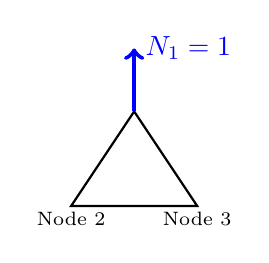
\begin{tikzpicture}[scale=0.8]
        \draw[thick] (0,0) -- (2,0) -- (1,1.5) -- cycle;
        \draw[->, blue, ultra thick] (1,1.5) -- (1,2.5) node[right]{$N_1=1$};
        \node at (0,-0.2) {\scriptsize Node 2};
        \node at (2,-0.2) {\scriptsize Node 3};
      \end{tikzpicture}
    \end{column}
  \end{columns}
\end{frame}

\begin{frame}{Calculation Method: Assembly and Eigen-solution}
  \begin{block}{Global Matrix Construction}
    Substituting the expansion into the Weak Form leads to the local element matrices:
    \begin{equation}
      \mathbf{k}^e_{ij} = \int_{\Omega_e} \frac{\hbar^2}{2m} \nabla N_i \cdot \nabla N_j + N_i V N_j \d \Omega_e, \quad \mathbf{m}^e_{ij} = \int_{\Omega_e} N_i N_j \d \Omega_e
    \end{equation}
  \end{block}
  \pause
  \begin{alertblock}{Final System}
    Summing all local contributions (Assembly) yields the global generalized eigenvalue problem:
    \begin{equation}
      \mathbf{K} \bm \Psi = E \mathbf{M} \bm \Psi
    \end{equation}
    
    Where $\mathbf{K}$ is the global \textbf{Stiffness Matrix} and $\mathbf{M}$ is the \textbf{Mass Matrix}.
  \end{alertblock}
\end{frame}

\section{METHODOLOGY}

\begin{frame}{Transition: From Tight-Binding to FEA}
  \begin{columns}
    \begin{column}{.48\linewidth}
      \centering \textbf{Tight-Binding (Discrete)}
      \begin{itemize}
        \item \textit{Basis:} Atomic orbitals at sites $A, B, C$.
        \item \textit{Interaction:} Hopping integrals $t_{ij}$.
        \item \textit{Hamiltonian:} $3 \times 3$ Matrix.
      \end{itemize}
    \end{column}
    \hfill
    \vrule
    \hfill
    \begin{column}{.48\linewidth}
      \centering \textbf{FEA (Continuous)}
      \begin{itemize}
        \item \textit{Basis:} Piecewise polynomials on a mesh.
        \item \textit{Interaction:} Potential field $V(\bm r)$.
        \item \textit{Hamiltonian:} Large sparse matrices $\mathbf{K}, \mathbf{M}$.
      \end{itemize}
    \end{column}
  \end{columns}
  \pause
  \begin{alertblock}{Governing Equation}
    Solve the time-independent Schrödinger equation:
    \begin{equation}
      \ab[-\frac{\hbar^2}{2m} \nabla^2 + V(\bm r)] \psi(\bm r) = E \psi(\bm r)
    \end{equation}
    where $V(\bm r)$ is the periodic potential of the Kagome lattice.
  \end{alertblock}
\end{frame}

\begin{frame}[allowframebreaks]{The Kagome Unit Cell Mesh}
  \begin{block}{Defining the Domain}
    For FEA, we define the unit cell containing three atoms (represented as cylinders/wells).
  \end{block}
  \begin{figure}[htbp]
    \centering
    \setbox0=\hbox{%
      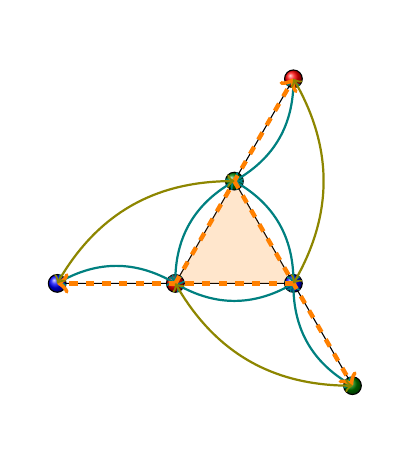
\begin{tikzpicture}[scale = .75]
        \path (-2.5,{2.5*sqrt(3)}) rectangle (3.5,{-1.5*sqrt(3)});
        \draw (2,0) -- (-2,0)
              (0,0) -- (2,{2*sqrt(3)})
              (1,{sqrt(3)}) -- (3,{-sqrt(3)});
        \fill [orange, opacity = .2] (0,0) -- (1,{sqrt(3)}) -- (2,0) -- cycle;
        \shade [draw, ball color = blue] (2,0) circle (.15) coordinate (A);
        \shade [draw, ball color = red] (0,0) circle (.15) coordinate (B);
        \shade [draw, ball color = Green] (1,{sqrt(3)}) circle (.15)
        coordinate (C);
        \shade [draw, ball color = blue] (-2,0) circle (.15)
        coordinate (A');
        \shade [draw, ball color = red] (2,{2*sqrt(3)}) circle (.15)
        coordinate (B');
        \shade [draw, ball color = Green] (3,{-sqrt(3)}) circle (.15)
        coordinate (C');
        \draw [thick, <->, teal] (A) to[bend left]  (B);
        \draw [thick, <->, teal] (B) to[bend left]  (C);
        \draw [thick, <->, teal] (C) to[bend left]  (A);
        \draw [thick, <->, teal] (B) to[bend right] (A');
        \draw [thick, <->, teal] (C) to[bend right] (B');
        \draw [thick, <->, teal] (A) to[bend right] (C');
        \draw [ultra thick, dashed, ->, orange] (B) -- (B');
        \draw [ultra thick, dashed, ->, orange] (A) -- (A');
        \draw [ultra thick, dashed, ->, orange] (C) -- (C');
        \draw [thick, <->, olive] (A) to[bend right] (B');
        \draw [thick, <->, olive] (B) to[bend right] (C');
        \draw [thick, <->, olive] (C) to[bend right] (A');
      \end{tikzpicture}
    }
    \begin{tikzpicture}[baseline, scale = 1.2]
      \node [inner sep = 0pt, scale = .6] at (0,0) {\usebox0};
      \node [inner sep = 0pt, scale = .6] at (1.5,0) {\usebox0};
      \node [inner sep = 0pt, scale = .6] at (-1.5,0) {\usebox0};
      \node [inner sep = 0pt, scale = .6] at (.75,{.75*sqrt(3)}) {\usebox0};
      \node [inner sep = 0pt, scale = .6] at (-.75,{.75*sqrt(3)}) {\usebox0};
    \end{tikzpicture}
    \enspace \textrightarrow \quad
    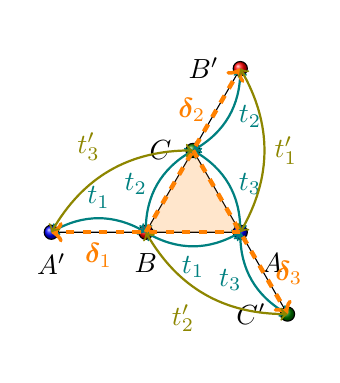
\begin{tikzpicture}[baseline, scale = .6]
      \path (-2.5,{2.5*sqrt(3)}) rectangle (3.5,{-1.5*sqrt(3)});
      \draw (2,0) -- (-2,0)
            (0,0) -- (2,{2*sqrt(3)})
            (1,{sqrt(3)}) -- (3,{-sqrt(3)});
      \fill [orange, opacity = .2] (0,0) -- (1,{sqrt(3)}) -- (2,0) -- cycle;
      \shade [draw, ball color = blue] (2,0) circle (.15) coordinate (A)
      node [below right = .15cm] {$A$};
      \shade [draw, ball color = red] (0,0) circle (.15) coordinate (B)
      node [below = .15cm] {$B$};
      \shade [draw, ball color = Green] (1,{sqrt(3)}) circle (.15)
      coordinate (C) node [left = .15cm] {$C$};
      \shade [draw, ball color = blue] (-2,0) circle (.15)
      coordinate (A') node [below = .15cm] {$A'$};
      \shade [draw, ball color = red] (2,{2*sqrt(3)}) circle (.15)
      coordinate (B') node [left = .15cm] {$B'$};
      \shade [draw, ball color = Green] (3,{-sqrt(3)}) circle (.15)
      coordinate (C') node [left = .15cm] {$C'$};
      \draw [thick, <->, teal] (A) to[bend left] node [below] {$t_1$} (B);
      \draw [thick, <->, teal] (B) to[bend left] node [left] {$t_2$} (C);
      \draw [thick, <->, teal] (C) to[bend left] node [right] {$t_3$} (A);
      \draw [thick, <->, teal] (B) to[bend right] node [above] {$t_1$} (A');
      \draw [thick, <->, teal] (C) to[bend right] node [right] {$t_2$} (B');
      \draw [thick, <->, teal] (A) to[bend right] node [left] {$t_3$} (C');
      \draw [ultra thick, dashed, ->, orange] (B) --
      node [left, near end] {$\bm \delta_2$} (B');
      \draw [ultra thick, dashed, ->, orange] (A) --
      node [below, near end] {$\bm \delta_1$} (A');
      \draw [ultra thick, dashed, ->, orange] (C) --
      node [right, near end] {$\bm \delta_3$} (C');
      \draw [thick, <->, olive] (A) to[bend right]
      node [right] {$t_1'$} (B');
      \draw [thick, <->, olive] (B) to[bend right]
      node [below left] {$t_2'$} (C');
      \draw [thick, <->, olive] (C) to[bend right]
      node [above left] {$t_3'$} (A');
    \end{tikzpicture}
    \caption{TB model of the Kagome unit cell.}
    \zlabel{fig:NNN_splice}
  \end{figure}
  \begin{figure}[htbp]
    \begin{minipage}{.56\linewidth}
      \centering
      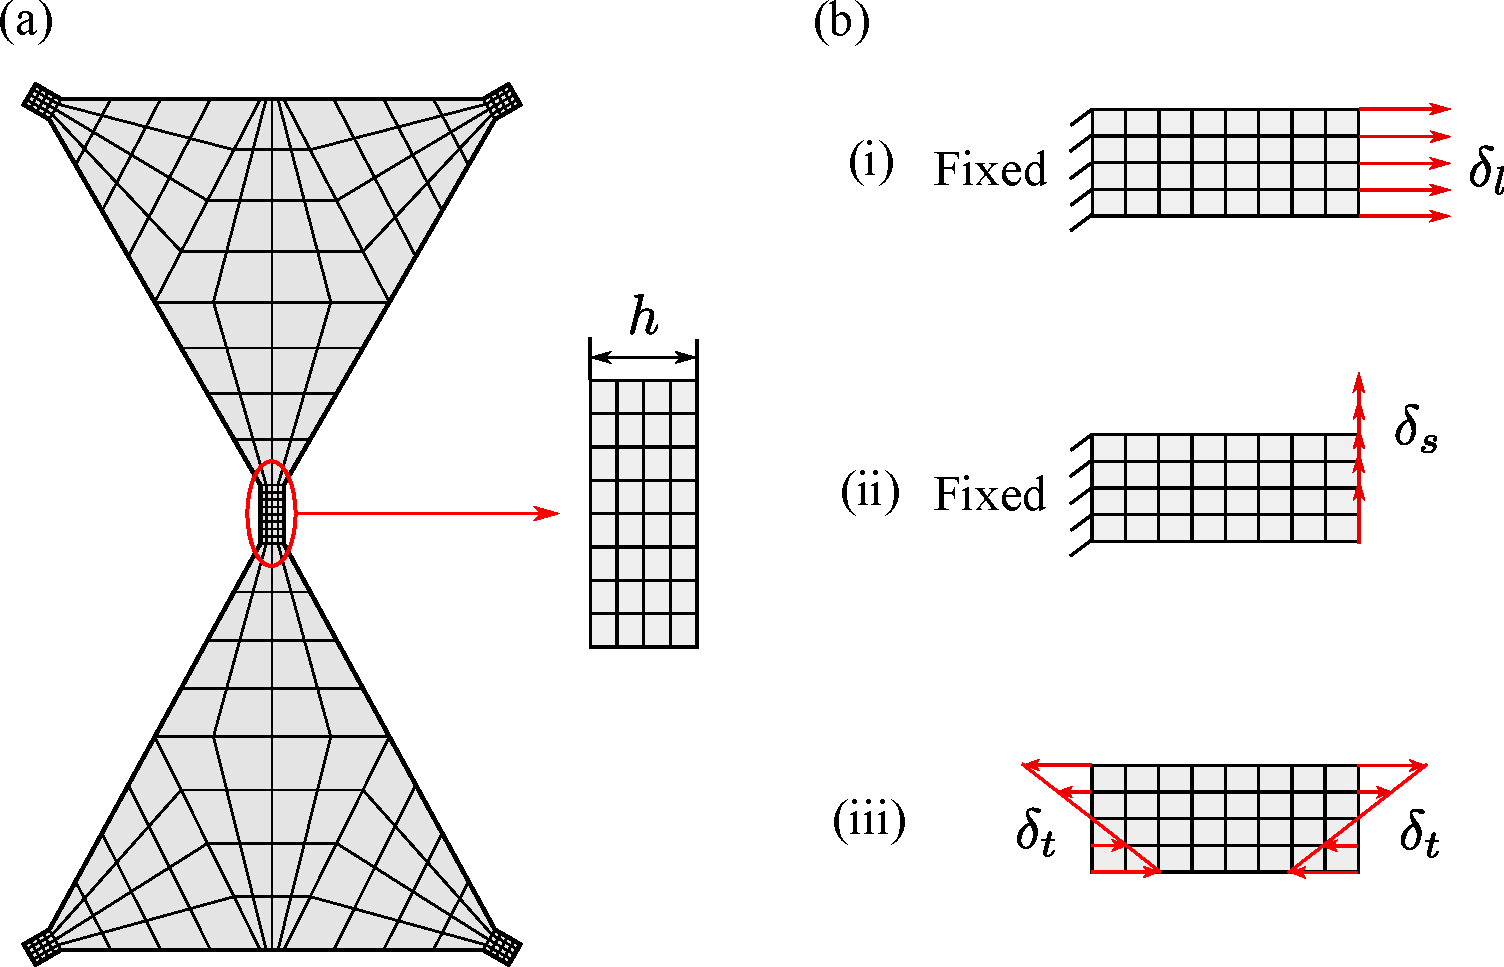
\includegraphics[height = .6\textheight]{Finite_element_model.pdf}
    \end{minipage}
    \hfill
    \begin{minipage}{.4\linewidth}
      \begin{itemize}
        \item (a) Meshing of the unit cell with an inset highlighting the ligament.
        \item (b) Schematics of the boundary conditions in the FE simulations to determine the equivalent
        \begin{itemize}
          \item longitudinal,
          \item shear, and
          \item torsional stiffnesses
        \end{itemize}
        of the ligament.
      \end{itemize}
    \end{minipage}
    \bigskip
    \caption{Mesh of Kagome unit cell. Each site is a local potential well.}
  \end{figure}
\end{frame}

\section{RESULT DISCUSSION}

\begin{frame}{Energy Bands via Eigenvalue Analysis}
  \begin{block}{Bloch Eigenvalue Problem}
    By applying $\psi(\bm r + \bm a_i) = \upe^{\iu \bm k \cdot \bm a_i} \psi(\bm r)$ to the mesh boundaries, the FEA matrices become $\bm k$-dependent:
    \begin{equation}
      \mathbf K(\bm k) \bm \psi = E(\bm k) \mathbf M \bm \psi,
    \end{equation}
    where $\bm k = (k_x, k_y, k_z)$ stands for the wavevector.
  \end{block}
  \pause
  \begin{exampleblock}{Comparing Results}
    \begin{itemize}
      \item \textbf{Tight-Binding:} Predicts a flat band and two dispersive bands.
      \item \textbf{FEA:} Recovers the same structure in the low-energy limit, but also shows \textbf{higher energy bands} (excited states) not captured by simple tight-binding models.
    \end{itemize}
  \end{exampleblock}
\end{frame}

\begin{frame}{Band Structure Visualization}
  \begin{block}{Trivial case}
    Simply taking $t_1 = t_2 = t_3 = t$
    \begin{equation}
      E_\pm
    = t\ab[-1 \pm \sqrt{\textstyle 3 + 2\sum_i^3
      \cos(\bm k \cdot \bm\delta_i)}], \quad
      E_\text{flat} = 2t
      \label{eq:band}
    \end{equation}
  \end{block}
  \pause
  \begin{exampleblock}{Numerical plotting}
    \begin{figure}[htbp]
      \begin{minipage}{.22\linewidth}
        \centering
        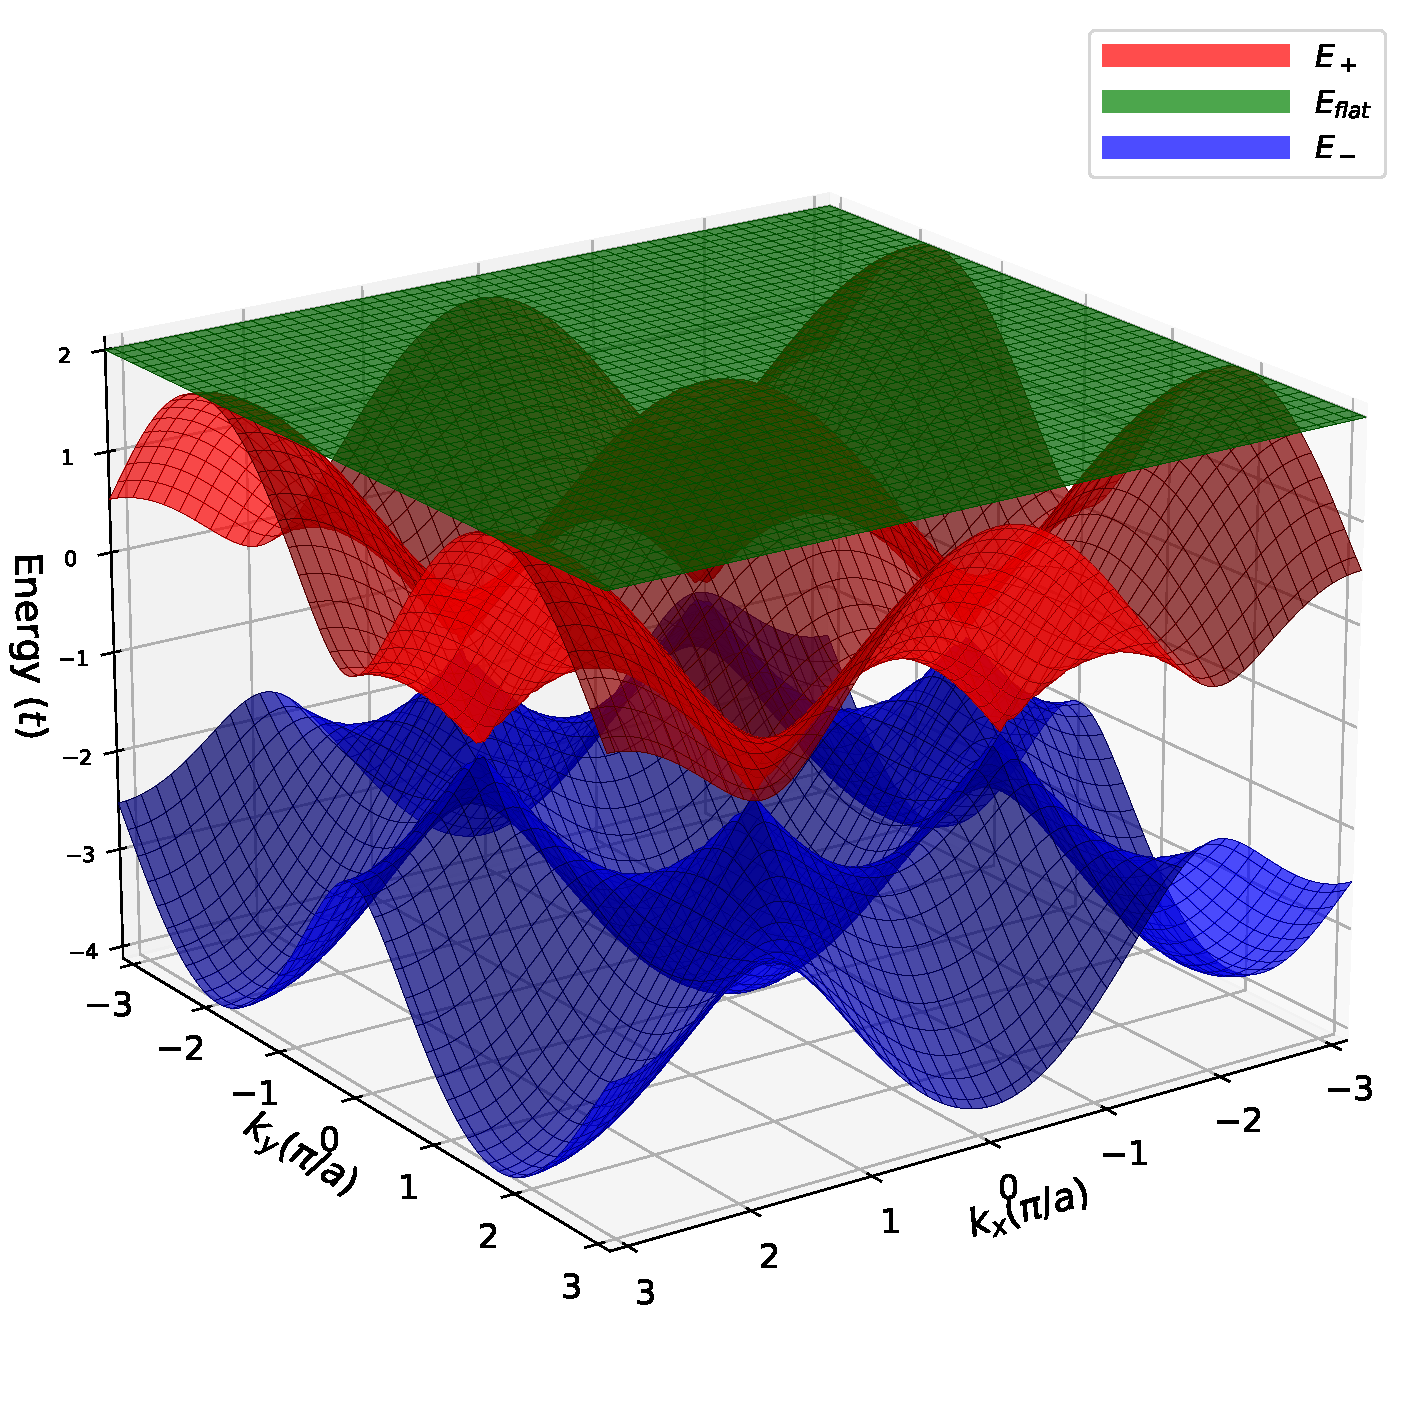
\includegraphics[page = 1, height = .32\paperheight]{kagome_bands.pdf}
      \end{minipage}
      \hfill
      \begin{minipage}{.22\linewidth}
        \centering
        \includegraphics[page = 2, height = .32\paperheight]{kagome_bands.pdf}
      \end{minipage}
      \hfill
      \begin{minipage}{.26\linewidth}
        \centering
        \includegraphics[page = 3, height = .32\paperheight]{kagome_bands.pdf}
      \end{minipage}
      \hfill
      \begin{minipage}{.26\linewidth}
        \centering
        \includegraphics[page = 4, height = .32\paperheight]{kagome_bands.pdf}
      \end{minipage}
      \caption{3D/2D Band structure for NN hopping under different perspectives
        computed via FEA.}
      \zlabel{fig:3Dband}
    \end{figure}
  \end{exampleblock}
\end{frame}

\section{ADVANCED STUDY}

\begin{frame}{Geometric Effects in FEA}
  Unlike Tight-Binding, where hopping $t$ is an abstract parameter, FEA allows us to study the effect of the \textbf{physical shape} of the lattice sites:
  \begin{itemize}
    \item \textbf{Site Radius:} How the band gap changes with atom size.
    \item \textbf{Potential Depth:} The transition from nearly-free electrons to strongly bound states.
    \item \textbf{Structural Defects:} Removing elements from the mesh to simulate vacancies.
  \end{itemize}
\end{frame}

\begin{frame}[t]{References}
  \nocite{*}
  \printbibliography
\end{frame}

\section{Thanks for Listening! Any Questions?}

\end{document}